\subsection{Implemented requirements}
\hspace{\parindent} The list of requirements and their implementation status is included in ITD file. Testing has been done on these implementations and the comments on whether they are correctly implemented or not are next to the requirement name in the following list:

\begin{itemize}
\item[\textbf{R.1}]\textbf{ The system shall allow customers to line-up remotely in a store queue.}\newline \textbf{Implementation status}: Implemented\newline \textbf{Comments}: The line-up implementation doesn't really exist, queueing is not managed by the time the ticket has been requested or the ticket number, but rather every ticket scan is accepted, making the store employee in charge for the decision on who can enter the store and not the system. The virtual line-up exists, but it's not ordered in any way, making the whole point of the line-up non existent.
\item[\textbf{R.2}] \textbf{The system shall generate a new ticket when a customer enters a queue}\newline \textbf{Implementation status}: Implemented\newline \textbf{Comments}: Implementation tested and working correctly.
\item[\textbf{R.3}]\textbf{The system shall allow customers which do not have a smartphone to get a ticket in place.}\newline \textbf{Implementation status}: Not implemented\newline \textbf{Comments}: /
\item[\textbf{R.4}]\textbf{The system shall allow customers to view the number of people lined up in a queue}\newline \textbf{Implementation status}: Implemented\newline \textbf{Comments}: Implementation tested and working correctly.
\item[\textbf{R.5}]\textbf{The system shall give customers an estimated waiting time.}\newline \textbf{Implementation status}:Partially implemented\newline \textbf{Comments}: Time estimation is equal to 1 person per 15 minutes. The estimation doesn't really work correctly since there is no store queueing and no way or determining how many people are in front, making estimation always be either 0 or 15 minutes.
\item[\textbf{R.6}]\textbf{The system shall fetch the GPS position while the user has retrieved a store pass.}\newline \textbf{Implementation status}:Not implemented\newline \textbf{Comments}: /
\item[\textbf{R.7}]\textbf{The system shall allow customers to leave a queue.}\newline \textbf{Implementation status}:Implemented\newline \textbf{Comments}: Customer can delete the ticket anytime, therefore leaving the queue. Implementation tested and working correctly.
\item[\textbf{R.8}]\textbf{The system shall allow customers to filter stores by name.}\newline \textbf{Implementation status}:Implemented\newline \textbf{Comments}: Implementation tested and working correctly.
\item[\textbf{R.9}]\textbf{The system shall notify customers when it’s time to leave for the store.}\newline \textbf{Implementation status}:Not implemented\newline \textbf{Comments}: /
\item[\textbf{R.10}]\textbf{The system shall allow customers to book-a-visit to the store and send them the confir-mation link and receipt via email.}\newline \textbf{Implementation status}:Not implemented\newline \textbf{Comments}: /
\item[\textbf{R.11}]\textbf{The system shall allow book-a-visit customers to specify the main categories of itemthey intend to buy.}\newline \textbf{Implementation status}:Not implemented\newline \textbf{Comments}: /
\item[\textbf{R.12}]\textbf{The system shall allow customers to delete a store pass.}\newline \textbf{Implementation status}:Partially implemented \newline \textbf{Comments}: There are no bookings because "Book a visit" feature doesn't exist. Ticket deletion working correctly.
\item[\textbf{R.13}]\textbf{The system shall notify customers when a ticket or booked visit is deleted.}\newline \textbf{Implementation status}:Not implemented\newline \textbf{Comments}: /
\item[\textbf{R.14}]\textbf{The system shall accept bookings based onto the already booked category items.}\newline \textbf{Implementation status}:Not implemented\newline \textbf{Comments}: /
\item[\textbf{R.15}]\textbf{The system shall allow a registered store manager to login by using their credentials.}\newline \textbf{Implementation status}:Implemented\newline \textbf{Comments}: Implementation tested and working correctly.
\item[\textbf{R.16}]\textbf{The system shall allow store managers to view the current status of people inside the store.}\newline \textbf{Implementation status}:Implemented\newline \textbf{Comments}: Implementation tested and working correctly.
\item[\textbf{R.17}]\textbf{The system shall allow store managers to view the current status of people in the queue.}\newline \textbf{Implementation status}:Implemented\newline \textbf{Comments}: Implementation tested and working correctly.
\item[\textbf{R.18}]\textbf{The system shall allow store managers to view the booked visits to the store.}\newline \textbf{Implementation status}:Not implemented\newline \textbf{Comments}: /
\item[\textbf{R.19}]\textbf{The system shall allow store managers to set a maximum cap of people inside the store.}\newline \textbf{Implementation status}:Implemented\newline \textbf{Comments}: Implementation tested and working correctly.
\item[\textbf{R.20}]\textbf{The system shall allow store managers to delete tickets and booked visits.}\newline \textbf{Implementation status}:Partially implemented \newline \textbf{Comments}: There are no bookings because "Book a visit" feature doesn't exist. Ticket deletion working correctly.
\item[\textbf{R.21}]\textbf{The system shall allow a registered store employee to login by using their credentials.}\newline \textbf{Implementation status}:Implemented \newline \textbf{Comments}: Implementation tested and working correctly.
\item[\textbf{R.22}]\textbf{The system shall allow store employee to view the current status of people inside the store.}\newline \textbf{Implementation status}:Implemented \newline \textbf{Comments}: Implementation tested and working correctly.
\item[\textbf{R.23}]\textbf{The system shall allow store employee to view the current status of people in the queue.}\newline \textbf{Implementation status}:Implemented \newline \textbf{Comments}: Implementation tested and working correctly.
\item[\textbf{R.24}]\textbf{The system shall allow store employee to scan QR codes.}\newline \textbf{Implementation status}:Implemented \newline \textbf{Comments}: Implementation tested and working correctly.
\item[\textbf{R.25}]\textbf{The system shall allow store employee to validate store passes.}\newline \textbf{Implementation status}:Partially implemented \newline \textbf{Comments}: there are no bookings because "Book a visit" feature doesn't exist. Ticket scanning working correctly.
\item[\textbf{R.26}]\textbf{The system shall allow CLup admins to register new supermarkets.}\newline \textbf{Implementation status}:Implemented \newline \textbf{Comments}: Implementation tested and working correctly. New supermarkets can be registered with name, full address, image, and work hours. No two stores of the same name and faulty work hours can be registered.
\item[\textbf{R.27}]\textbf{The system shall generate new manager and staff credentials for each supermarket registered.}\newline \textbf{Implementation status}:Implemented \newline \textbf{Comments}: Implementation tested and working correctly.
\end{itemize}

We have also replicated (manually) all the Unit and System tests defined in ITD1.0.pdf file under chapters 5.1 and 5.3. We have gotten the same results as the creators of the system. Here are a couple of examples and error messages received when trying different "bad" actions.

\begin{figure}[!htb]
\centering
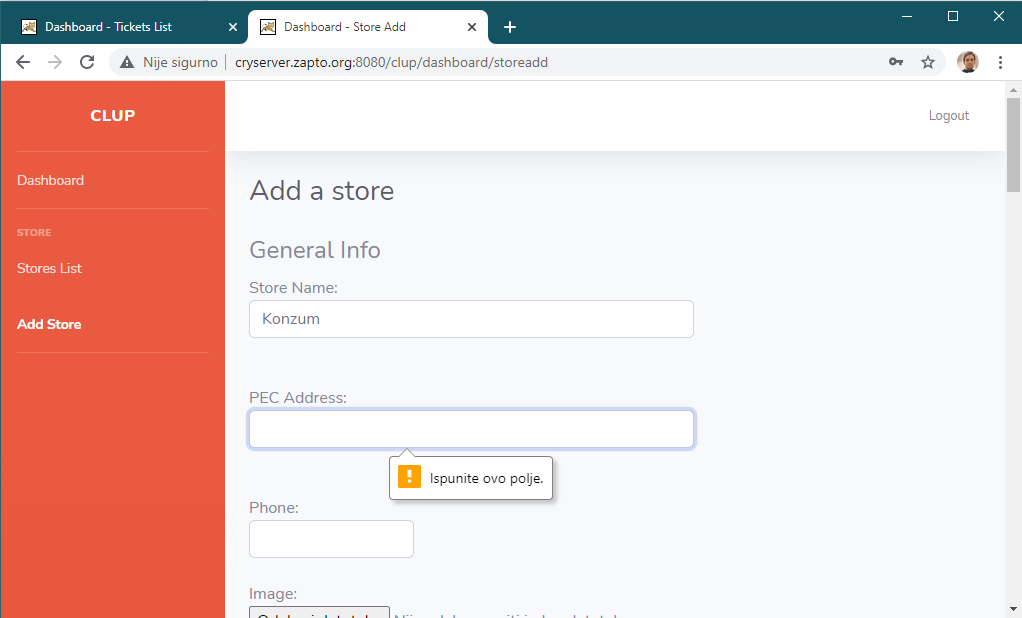
\includegraphics[width=\textwidth]{Images/FieldEmpty}
\captionsetup{justification=centering}
\caption{\label{fig:desktoperr1}\textbf{Left empty field when creating a store}}
\end{figure}
\begin{figure}[!htb]
\centering
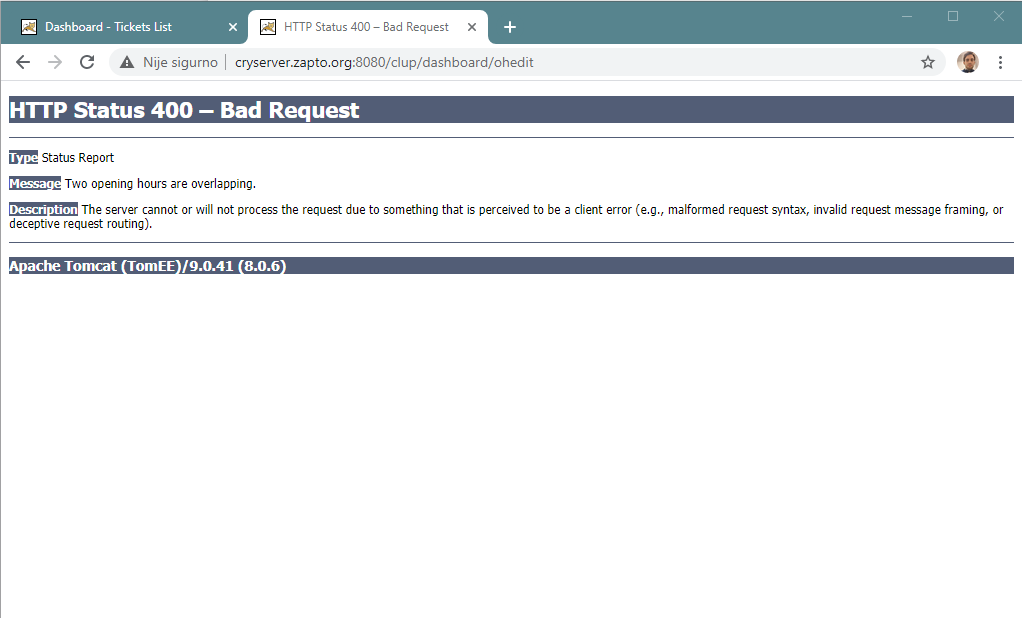
\includegraphics[width=\textwidth]{Images/BadHours}
\captionsetup{justification=centering}
\caption{\label{fig:desktoperr2}\textbf{Bad work hours written - two overlapping intervals}}
\end{figure}
\begin{figure}[!htb]
\centering
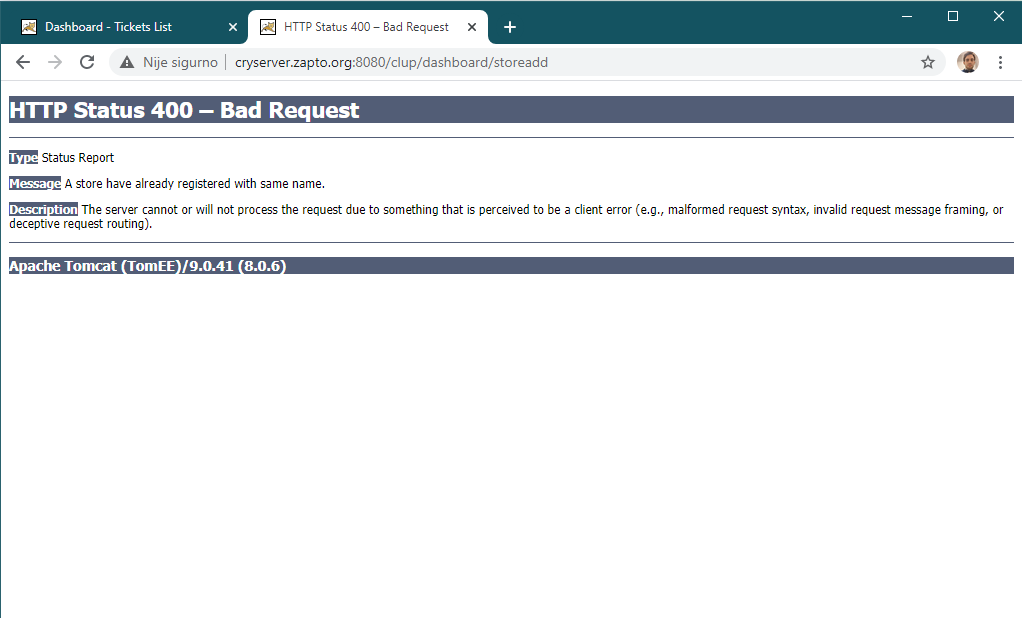
\includegraphics[width=\textwidth]{Images/SameName}
\captionsetup{justification=centering}
\caption{\label{fig:desktoperr3}\textbf{Two stores of the same name error}}
\end{figure}

\begin{figure}[!htb]
\centering
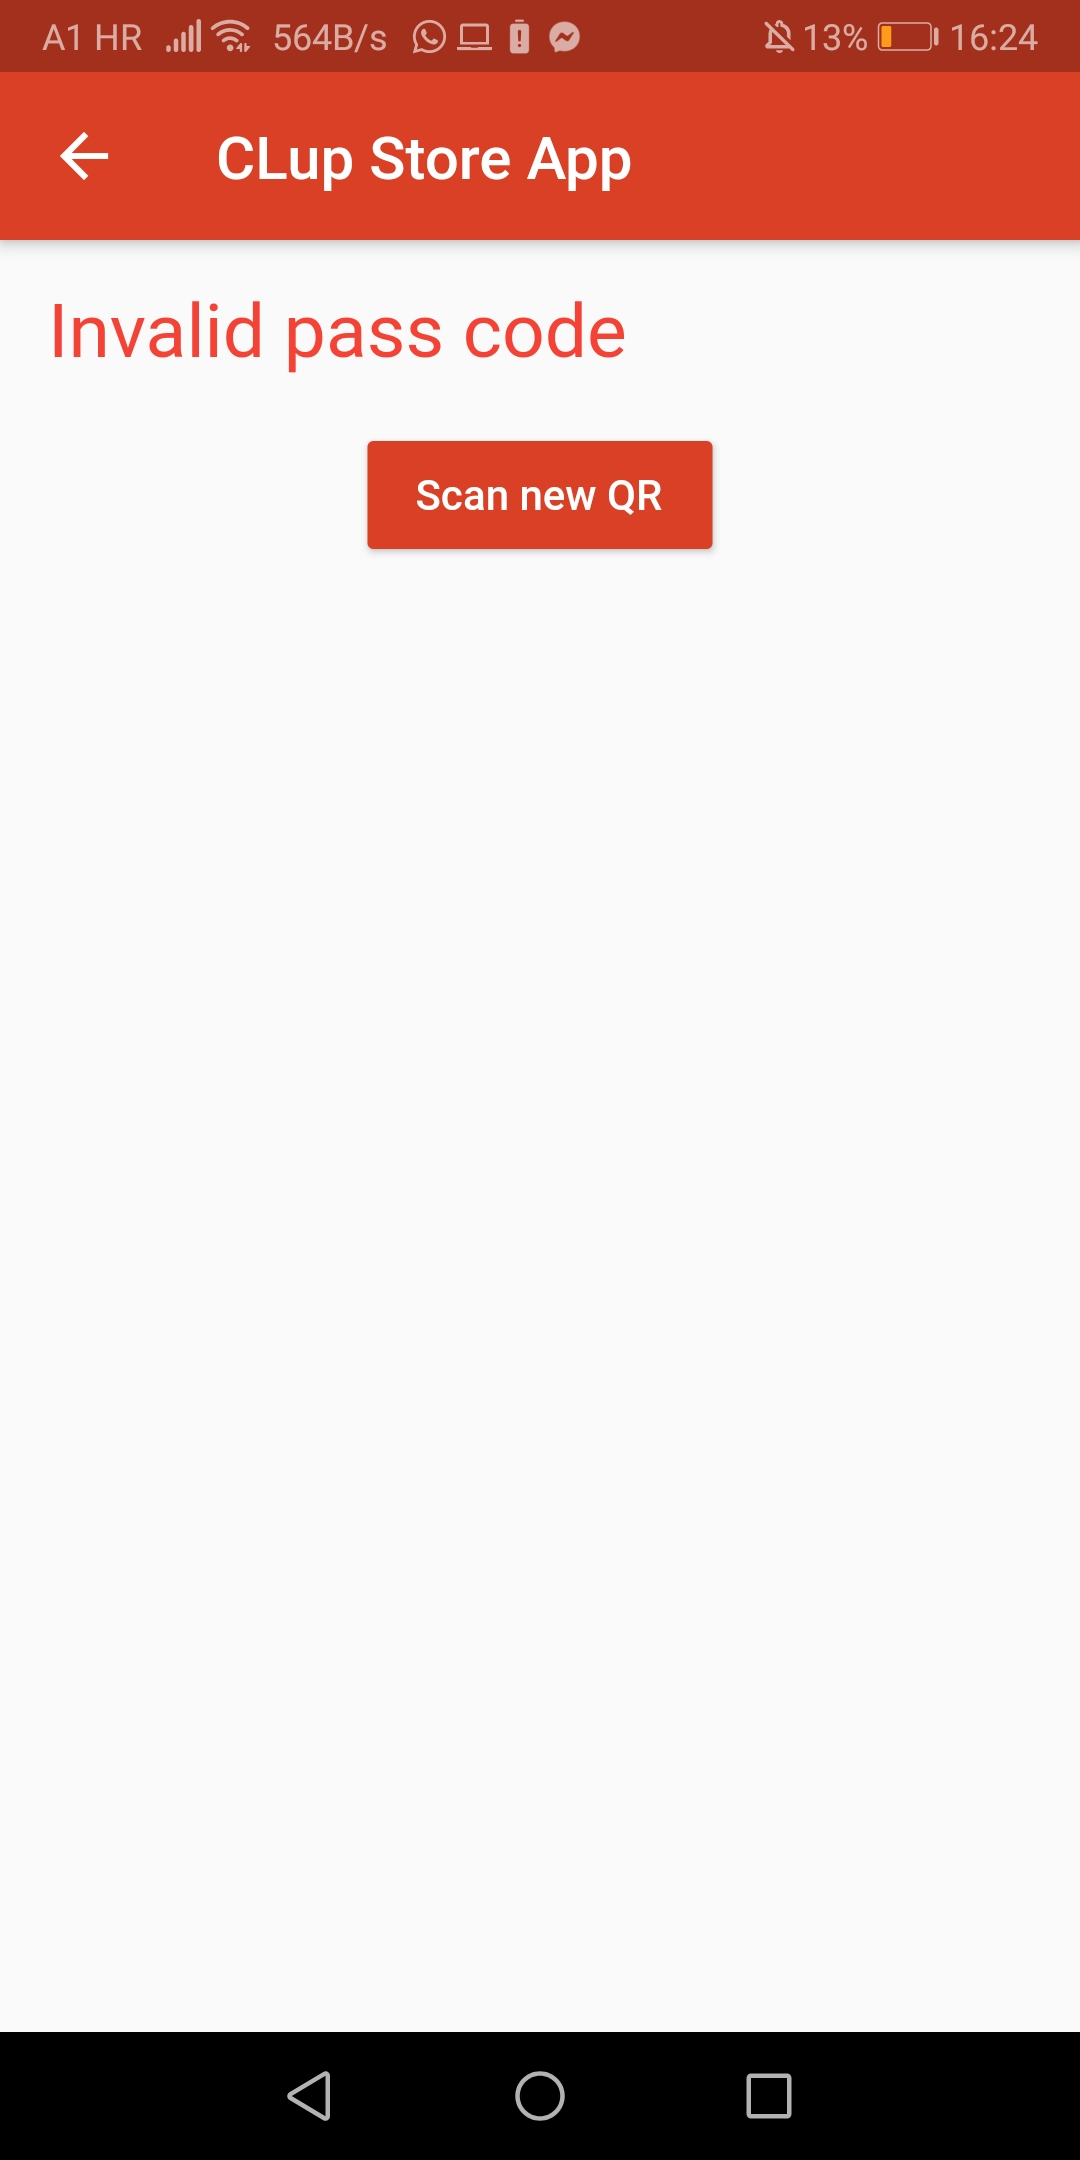
\includegraphics[width=0.35\textwidth]{Images/InvalidScan}
\captionsetup{justification=centering}
\caption{\label{fig:appandroiderr3}\textbf{Invalid QR code scan error}}
\end{figure}

\begin{figure}[!htb]
\centering
\begin{minipage}{0.45\textwidth}
\centering
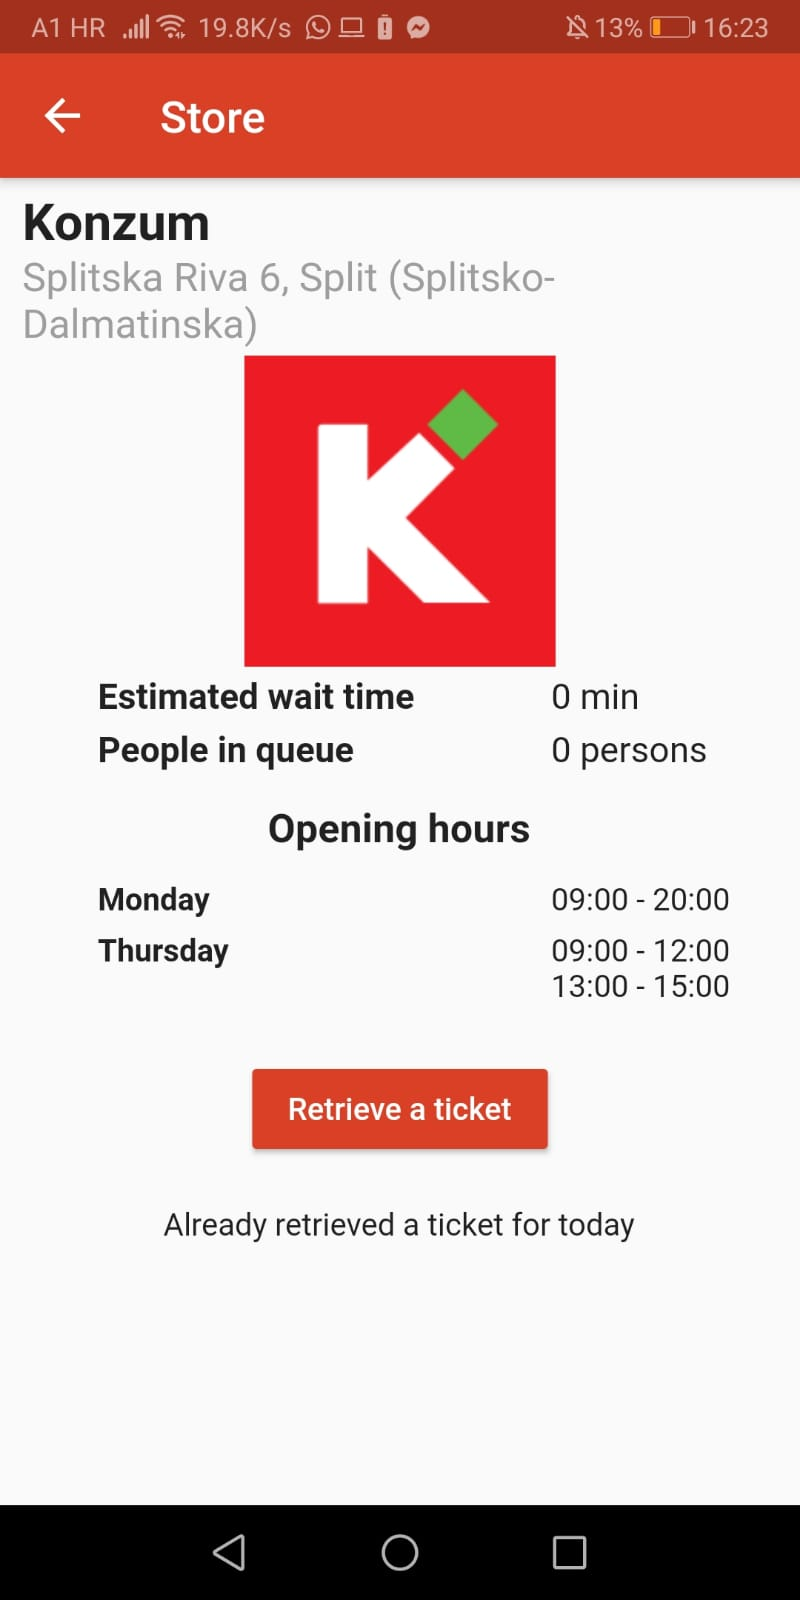
\includegraphics[width=0.9\textwidth]{Images/AlreadyRetrieved}
\captionsetup{justification=centering}
\caption{\label{fig:appandroiderr1}\textbf{Ticket already retrieved for the same store that day (and not deleted yet)}}
\end{minipage}
\begin{minipage}{0.45\textwidth}
\centering
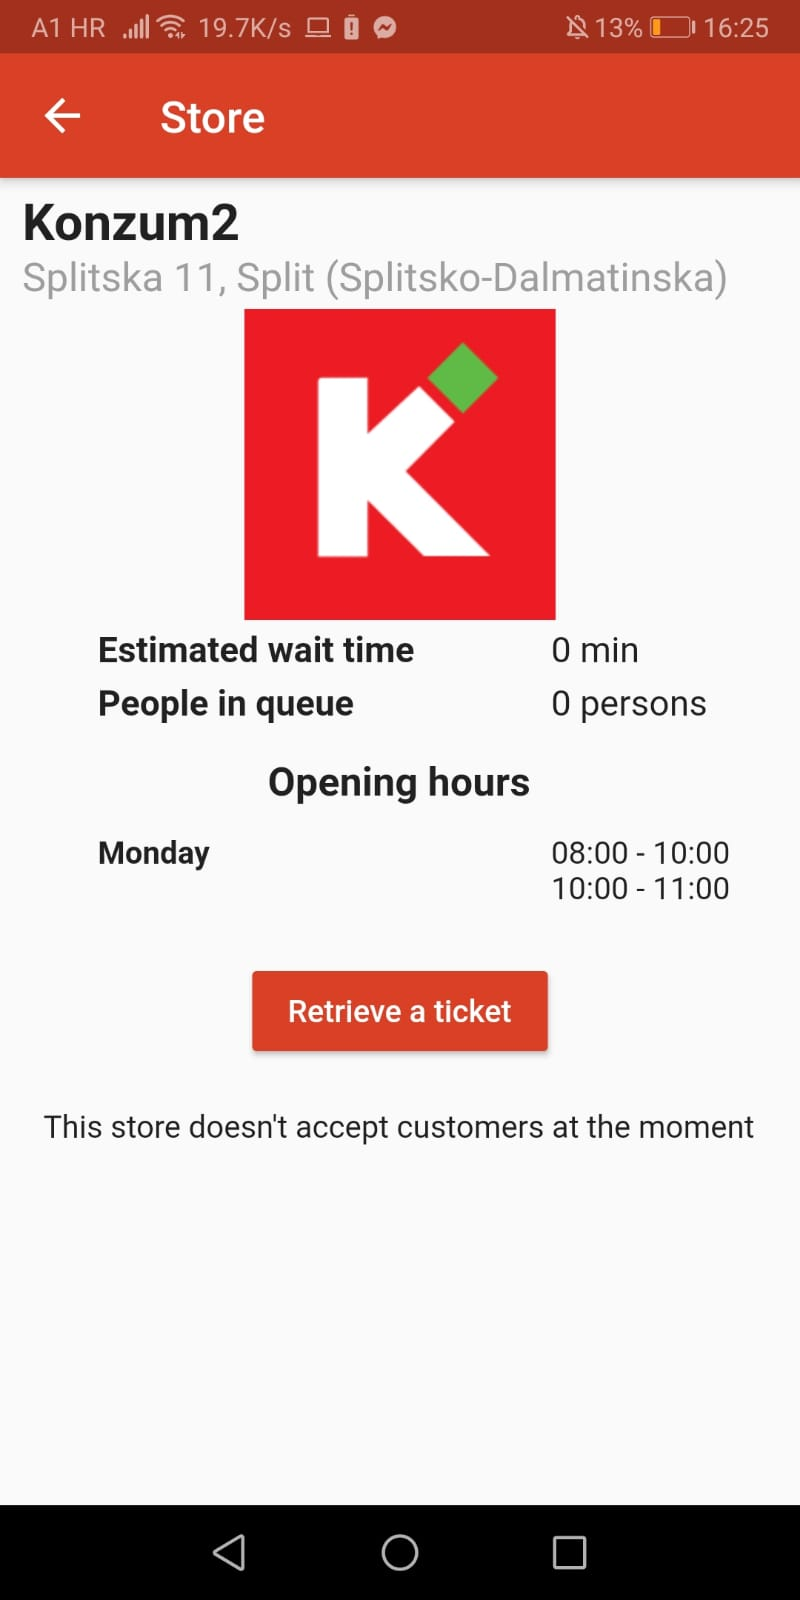
\includegraphics[width=0.9\textwidth]{Images/ClosedStore}
\captionsetup{justification=centering}
\caption{\label{fig:appandroiderr2}\textbf{The store is currently closed error}}
\end{minipage}
\end{figure}


